\section{Техническое задание}
\subsection{Основание для разработки}

Основанием для разработки является задание на выпускную квалификационную работу бакалавра "<Кроссплатформенная система обмена сообщениями">.

\subsection{Цель и назначение разработки}

Разрабатываемый программный продукт предназначен для организации общения пользователей приложения.

Пользователи данного приложения должны иметь возможность создавать свои комнаты для общения, управлять пользователями комнаты в соответствии со своими ролями, обмениваться голосовыми и текстовыми сообщениями, а также иметь возможность отправлять файлы.

Задачами данной разработки являются:
\begin{itemize}
\item проектирование архитектуры приложения;
\item реализация функциональности серверной части приложения;
\item реализация механизмов аутентификации и авторизации;
\item реализация клиентской части приложения;
\item тестирование и отладка.
\end{itemize}


\subsection{Функциональные требования к программной системе}

Для неавторизованных пользователей системы должны быть доступны следующие функции:

\begin{itemize}
	\item вход в приложение,
	\item регистрация.
\end{itemize}

Вне чат-комнаты авторизованным пользователям должны быть доступны следующие функции:
\begin{itemize}
	\item создание чат-комнаты,
	\item управление личными данными.
\end{itemize}
Внутри чат-комнаты предусмотрено наличие трех классов пользователей: администраторы чата, модераторы чата и обычные пользователи.

Администратором чата назначается пользователь, создавший чат. Он должен иметь следующие возможности:
\begin{itemize}
	\item добавление новых пользователей,
	\item удаление пользователей,
	\item удаление сообщений,
	\item удаление чата,
	\item управление ролями пользователей,
	\item отправка сообщений и файлов,
	\item редактирование своих сообщений.
\end{itemize}

Модераторы чата имеют те же возможности, что и администраторы, за исключением возможностей управления ролями пользователей и удаления чата.

Функции, доступные обычному пользователю:
\begin{itemize}
	\item добавление новых пользователей,
	\item удаление своих сообщений,
	\item отправка сообщений и файлов,
	\item редактирование своих сообщений.
\end{itemize}

\subsection{Моделирование вариантов использования}

Учитывая описанные ранее функцианальные требования к программной системе можно разработать модель вариантов использования системы.

Для составления данной модели используется язык визуального моделирования UML.

Данная описывает взаимодействие пользователей (актеров) с системой через варианты использования (use cases) для достижения определенной цели. В диаграмме выделяются актёры, варианты использования и связи между ними. Актёры представляют внешние сущности, взаимодействующие с системой, и обозначаются человечками или именем актёра. Варианты использования описывают функции или задачи системы и обозначаются овальными фигурами. Связи между актёрами и вариантами использования показывают, кто инициирует или участвует в конкретном варианте использования, и обозначаются линиями. Дополнительные элементы включают обобщение актёров, включение, расширение и системные границы, которые помогают уточнить и организовать функциональные требования системы. 

На рисунке \ref{unauth:image} в виде диаграммы прецедентов представлены функциональные требования к системе для неавторизованных пользователей.

На рисунке \ref{auth:image} в виде диаграммы прецедентов представлены функциональные требования к системе для авторизованных пользователей вне чат-комнаты.

На рисунке \ref{admin:image} в виде диаграммы прецедентов представлены функциональные требования к системе для авторизованных пользователей внутри чат комнаты для роли администратора чата. Построение отдельных диаграмм для остальных ролей не требуется, т.к. все прецеденты будут отражены на диаграмме прецедентов для роли администратора.

\begin{figure}[ht]
	\center{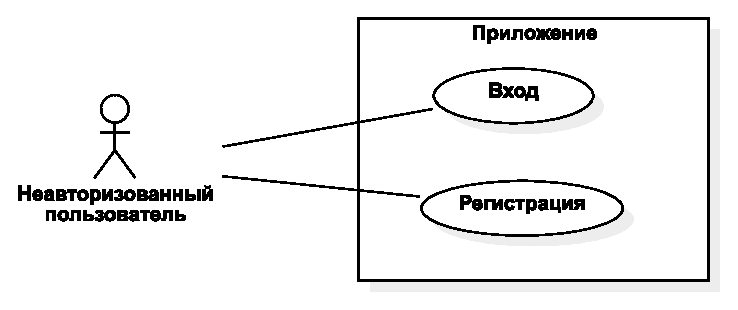
\includegraphics[width=1\linewidth]{unauth}}
	\caption{Диаграмма компонентов}
	\label{unauth:image}
\end{figure}
\ \\
\begin{figure}[ht]
	\center{\includegraphics[width=1\linewidth]{auth}}
	\caption{Диаграмма компонентов}
	\label{auth:image}
\end{figure}

\begin{figure}[H]
	\center{\includegraphics[width=1\linewidth]{admin}}
	\caption{Диаграмма компонентов}
	\label{admin:image}
\end{figure}

\subsubsection{Вариант использования "<Вход в приложение">}

Заинтересованные лица и их требования: пользователи, желающие получить доступ к функционалу приложения.

Предусловие: пользователь открыл приложение и находится на экране входа, пользователь зарегистрирован в приложении.

Постусловие: после успешной авторизации пользователь получает доступ к функциям приложения.

Основной успешный сценарий:
\begin{enumerate}
	\item Пользователь открывает приложение и переходит на экран входа.
	\item Пользователь вводит свои учетные данные (логин и пароль) в соответствующие поля.
	\item Приложение проверяет введенные учетные данные на корректность.
	\item При успешной проверке приложение авторизует пользователя и перенаправляет его на главный экран приложения.
\end{enumerate}

\subsubsection{Вариант использования "<Регистрация">}

Заинтересованные лица и их требования: пользователи, желающие получить доступ к функционалу приложения.

Предусловие: пользователь открыл приложение и находится на экране регистрации, пользователь не зарегистрирован в приложении.

Постусловие: пользователь получает доступ к созданной им чат-комнате.

Основной успешный сценарий:

\begin{enumerate}
	\item Пользователь запускает приложение и переходит на экран регистрации.
	\item Пользователь вводит нкобходимые для регистрации данные.
	\item Приложение проверяет введенные данные на корректность и уникальность.
	\item При успешной проверке приложение создает новую учетную запись для пользователя.
	\item Пользователь получает подтверждение успешной регистрации и может авторизоваться в системе используя свои учетные данные.
\end{enumerate}

\subsubsection{Вариант использования "<Создание чат-комнаты">}

Заинтересованные лица и их требования: пользователь хочет создать собственную чат-комнату для общения.

Предусловие: пользователь открыл приложение и находится на основном экране приложения, пользователь успешно прошел авторизацию.

Постусловие: после успешной регистрации пользователь получает доступ к функциям приложения.

Основной успешный сценарий:

\begin{enumerate}
	\item Пользователь открывает главный экран приложения.
	\item Пользователь выбирает опцию "Создать чат-комнату".
	\item Пользователь вводит название и указывает необходимые параметры.
	\item Приложение проверяет корректность введенных данных и создает новую чат-комнату.
	\item После успешного создания комнаты пользователь автоматически перенаправляется в нее.
\end{enumerate}

\subsubsection{Вариант использования "<Управление личными данными">}

Заинтересованные лица и их требования: пользователь хочет изменить свои данные, указанные при регистрации в приложении.

Предусловие: пользователь открыл приложение и находится в личном кабинете, пользователь успешно прошел авторизацию.

Постусловие: данные пользователя успешно изменены.

Основной успешный сценарий:

\begin{enumerate}
	\item Пользователь открывает главный экран приложения.
	\item Пользователь выбирает опцию "Страница пользователя".
	\item Пользователь производит необходимые изменения.
	\item Приложение проверяет корректность введенных данных и сохраняет изменения.
	\item Пользователь видит новые данные у себя на странице.
\end{enumerate}

\subsubsection{Вариант использования "<Добавление нового пользователя">}

Заинтересованные лица и их требования: пользователь хочет добавить нового участника в чат-комнату.

Предусловие: пользователь открыл приложение и находится в чат-комнате, пользователь успешно прошел авторизацию.

Постусловие: новый пользователь добавлен в чат-комнату.

Основной успешный сценарий:

\begin{enumerate}
	\item Пользователь открывает приложение и заходит в одну из доступных чат-комнат.
	\item Пользователь выбирает опцию "Добавить пользователя".
	\item Пользователь выбирает другого пользователя, которого хочет добавить в чат-комнату.
	\item Новый пользователь добавлен в чат-комнату.
\end{enumerate}

\subsubsection{Вариант использования "<Удаление пользователя">}

Заинтересованные лица и их требования: пользователь хочет удалить участника из чат-комнаты.

Предусловие: пользователь открыл приложение и находится в чат-комнате, пользователь успешно прошел авторизацию и имеет роль либо администратора, либо модератора.

Постусловие: выбранный пользователь удален из чат-комнаты.

Основной успешный сценарий:

\begin{enumerate}
	\item Пользователь открывает приложение и заходит в одну из доступных чат-комнат.
	\item Пользователь выбирает участника чата, которого хочет удалить и выбирает опцию "<Удалить пользователя">.
	\item Пользователь подтверждает свой выбор.
	\item Выбранный пользователь удален из чат-комнаты.
\end{enumerate}

\subsubsection{Вариант использования "<Удаление сообщения">}

Заинтересованные лица и их требования: пользователь хочет удалить свое сообщение в чате.

Предусловие: пользователь открыл приложение и находится в чат-комнате, пользователь успешно прошел авторизацию.

Постусловие: выбранное сообщение удалено из чата.

Основной успешный сценарий:

\begin{enumerate}
	\item Пользователь открывает приложение и заходит в одну из доступных чат-комнат.
	\item Пользователь выбирает сообщение, которое хочет удалить и выбирает опцию "<Удалить сообщение">.
	\item Пользователь подтверждает свой выбор.
	\item Выбранное сообщение удалено из чата.
\end{enumerate}

\subsubsection{Вариант использования "<Управление ролями пользователя">}

Заинтересованные лица и их требования: пользователь хочет изменить роль участника чат-комнаты.

Предусловие: пользователь открыл приложение и находится в чат-комнате, пользователь успешно прошел авторизацию и имеет роль администратора.

Постусловие: роль выбранного пользователя изменена.

Основной успешный сценарий:

\begin{enumerate}
	\item Пользователь открывает приложение и заходит в одну из доступных чат-комнат.
	\item Пользователь выбирает участника чата, роль которого хочет изменить и выбирает опцию "<Изменить роль">.
	\item Пользователь выбирает желаемую роль и подтверждает свой выбор.
	\item Роль выбранного пользователя изменена.
\end{enumerate}

\subsubsection{Вариант использования "<Удаление чата">}

Заинтересованные лица и их требования: пользователь хочет удалить созданную им чат-комнату.

Предусловие: пользователь открыл приложение и находится в чат-комнате, пользователь успешно прошел авторизацию и имеет роль администратора.

Постусловие: чат-комната удалена.

Основной успешный сценарий:

\begin{enumerate}
	\item Пользователь открывает приложение и заходит в одну из доступных чат-комнат.
	\item Пользователь выбирает опцию "<Удалить чат">.
	\item Пользователь подтверждает свой выбор.
	\item Чат-комната удалена и пользователь возвращается на главную страницу приложения.
\end{enumerate}

\subsubsection{Вариант использования "<Отправка сообщения">}

Заинтересованные лица и их требования: пользователь хочет отправить сообщение в чат.

Предусловие: пользователь открыл приложение и находится в чат-комнате, пользователь успешно прошел авторизацию.

Постусловие: сообщение отображется в чате.

Основной успешный сценарий:

\begin{enumerate}
	\item Пользователь открывает приложение и заходит в одну из доступных чат-комнат.
	\item Пользователь вводит сообщение в соответствующее поле и нажимает кнопку "<Отправить">.
	\item Сообщение пользователя отображается в чате.
\end{enumerate}

\subsubsection{Вариант использования "<Отправка голосового сообщения">}

Заинтересованные лица и их требования: пользователь хочет отправить голосовое сообщение в чат.

Предусловие: пользователь открыл приложение и находится в чат-комнате, пользователь успешно прошел авторизацию.

Постусловие: голосовое сообщение отображается в чате.

Основной успешный сценарий:

\begin{enumerate}
	\item Пользователь открывает приложение и заходит в одну из доступных чат-комнат.
	\item Пользователь нажмает кнопку "<Отправить голосовое сообщение"> и посредством микрофона устройства вводит сообщение голосом.
	\item Сообщение пользователя отображается в чате.
\end{enumerate}

\subsubsection{Вариант использования "<Редактирование сообщения">}

Заинтересованные лица и их требования: пользователь хочет отредактировать отправленное им сообщение.

Предусловие: пользователь открыл приложение и находится в чат-комнате, пользователь успешно прошел авторизацию.

Постусловие: в чате отображаетя отредактированное пользователем сообщение.

Основной успешный сценарий:

\begin{enumerate}
	\item Пользователь открывает приложение и заходит в одну из доступных чат-комнат.
	\item Пользователь выберает желаемое сообщение и выберает опцию "<Отредактировать">.
	\item Отредатированное пользователем сообщение отображается в чате.
\end{enumerate}

\subsubsection{Вариант использования "<Отправка файла">}

Заинтересованные лица и их требования: пользователь хочет отправить отправить в чат.

Предусловие: пользователь открыл приложение и находится в чат-комнате, пользователь успешно прошел авторизацию.

Постусловие: отправленый файл отображается в чате.

Основной успешный сценарий:

\begin{enumerate}
	\item Пользователь открывает приложение и заходит в одну из доступных чат-комнат.
	\item Пользователь нажмает кнопку "<Отправить файл"> и выберает нужный файл для отправки.
	\item Отправленный файл отображается в чате.
\end{enumerate}

\subsection{Требования к программному обеспечению}

Для работы клиентской части необходимо наличие браузера (Chrome от 64 версии, Microsoft Edge от версии 79 или аналогичные).
Для работы серверных компонентов требуется ОС семейства Linux или Windows c установленной СУБД PostgreSQL, .NET Core.

\subsection{Требования к оформлению документации}

Разработка программной документации и программного изделия должна производиться согласно ГОСТ 19.102-77 и ГОСТ 34.601-90. Единая система программной документации.
